\section{Future Work}


\subsection{Improve Robustness}
In this paper we have made many simplifications to the problem space just to make the placer easier to implement.
For example, our placer in its current state does not take advantage of \texttt{SLICEL}/\texttt{SLICEM} heterogeneity and simply maps all SLICE \texttt{SiteInst}s onto \texttt{SLICEL}s. 
Recall that the SLICE Sites in Xilinx FPGAs typically come in a 75-25\% split between \texttt{SLICEL}s and \texttt{SLICEM}s. 
This means that we have rendered about 25\% of the CLB fabric unusable which will inevitably hurt wirelength minimization during placement since the \texttt{SiteInst}s must be spread over a larger area. 
Enabling \texttt{SLICEL}-\texttt{SLICEM} heterogeneity can lead do greater logic density and consequently less total HPWL, but can make the packing process more complex and may contribute to higher routing congestion.

We can also add packing support for other Xilinx primitives such as the shift-register primitive \texttt{SRLx}, distributed RAM primitives \texttt{RAMSx}, or even \texttt{LATCH} primitives as discussed in \ref{sec:7_series}.
Adding support for additional primitives and macros will allow our placer to handle a wider range of HDL designs and will require deeper consideration of hardware constraints to ensure robustness.

In its current state, the prepacker and packer encounter problems when handling signals larger than 24-bits, especially when involved in DSP functions like addition and multiplication. 
In such designs, the Vivado synthesizer may synthesize long \texttt{CARRY4} chains with specific \texttt{EDIFHierPortInst} configurations which are currently not handled by our packer and lead to failures in the subsequent routing stage.
Further work is required to resolve these constraints in the packer.

\subsection{Analytical Placement}
As discussed earlier, simulated annealing (SA) has largely been phased out in state-of-the-art (SOTA) placers due to poor scalability and long runtimes. 
Our current placer follows a straightforward \emph{prepack–pack–place} flow, with the final placement stage driven by SA. 
In future work, this stage can be retrofitted to use analytical placement (AP) while reusing the prepacker and packer. 
Here, \texttt{SiteInst}s remain the atomic placement objects, and analytical solvers can be applied to minimize the total half-perimeter wirelength (HPWL) of the connecting nets.

The following works provide a foundation for understanding AP, ranging from early formulations to modern SOTA methods:
\begin{itemize}
    \item \emph{Analytical minimization of half-perimeter wirelength} — \textbf{Kennings and Markov (2000)} \cite{AP_2000}.
    \item \emph{Kraftwerk2—A Fast Force-Directed Quadratic Placement Approach Using an Accurate Net Model} — \textbf{Spindler et al. (2008)} \cite{kraftwerk2}.
    \item \emph{Analytical placement for heterogeneous FPGAs} — \textbf{Gort et al. (2012)} \cite{AP_2012}.
    \item \emph{SimPL: An algorithm for placing VLSI circuits} — \textbf{Kim et al. (2013)} \cite{SimPL}.
    \item \emph{Multi-Electrostatic FPGA Placement Considering SLICEL–SLICEM Heterogeneity, Clock Feasibility, and Timing Optimization} — \textbf{Jing et al. (2023)} \cite{MultiElectrostatic}.
    \item \emph{OpenPARF 3.0: Robust Multi-Electrostatics Based FPGA Macro Placement Considering Cascaded Macro Groups and Fence Regions} — \textbf{Jing et al. (2024)} \cite{OpenPARF}.
\end{itemize}

As noted in Section~\ref{sec:placement}, replacing SA with AP requires splitting the placement stage into two substages:  
\emph{global placement}, which determines continuous target positions using analytical optimization, and  
\emph{detailed placement} (legalization), which snaps objects to valid \texttt{site}s while adhering to hardware constraints.  
Global placement can be performed using any number of off-the-shelf (OTS) analytical solvers, but detailed placement requires custom implementation tailored to the hardware.
We repeatedly loop through global placement into detailed placement until HPWL minimization slows to a stop.

Unlike SA, which primarily relies on heuristics and probabilistic moves, AP begins by contextualizing the problem as a collection of mathematical expressions compatible with convex optimization solvers.
As briefly introduced in Section~\ref{subsec:netlist}, a circuit netlist can be naturally modeled as a hypergraph
\begin{equation}
    G_{H} = (V_{H}, E_{H})
    \label{equ:hypergraph}
\end{equation}
where \(V_{H}\) is the set of vertices and \(E_{H}\) is the set of hyperedges, each of which may connect more than two vertices. 
In RapidWright context, \(V_{H}\) corresponds to the set of \texttt{SiteInst}s placed on the \texttt{device}, while \(E_{H}\) corresponds to the set of \texttt{Net}s connecting them.
More accurately, $V_H$ corresponds to the set of pins (\texttt{SitePinInst}, or SPI for short), not the \texttt{SiteInst}s themselves.
The distinction is usually only important in VLSI context, when the area of a module or macro instance is large enough that the distance between its pins becomes significant \cite{kraftwerk2}.
However, in the context of FPGAs where \texttt{Site}s are relatively uniform size and whose areas are small compared to the area of the \texttt{device}, all \texttt{SitePinInst}s belonging to the same \texttt{SiteInst} can share the same location coordinates.


This hypergraph can be reduced into a graph using one of several net models:
\begin{itemize}
    \item \textbf{Star model:} classically, introduce a virtual star node and connect it to all pins of the net. However, in electronics, we can simply use the voltage source node as the star node and avoid adding virtual nodes.
    \item \textbf{Clique model:} connect all pins of the net to each other (quadratic growth in edges). 
    \item \textbf{Bound2Bound (B2B) model:} connect only the pins at the geometric boundary (min/max in $x$ or $y$) to each other, and connect boundary pins to all interior pins. With inverse-distance weights, this model matches HPWL exactly at the point of weight calculation.
\end{itemize}

% The VLSI placer Kraftwerk2 (2008) \cite{kraftwerk2} uses the following notation.
% Integrated circuits consist of a set of modules (set $M$), the modules have pins (set $P$), and the pins are connected by nets (set $N$).
% The nets are modeled by 2-pin connections 
% After hypergraph reduction using one of the net models, this results in the representation of each net $n \in N$ by a set $\mathcal{E}_n$ of 2-pin connections. 
% A single 2-pin connection $e = (p, q)$ connects pins $p$ and $q$.
% Each pin, $p$ for example, is located at coordinates $(x_p, y_p)$.

Since HPWL is direction-agnostic, directionality of FPGA nets (source/sinks) is typically ignored in reduction. 
Figure \ref{fig:net_model} shows an example of hyperedge reduction using the star and clique models while \ref{fig:bound2bound} shows the B2B reduction.

\vspace{1.0cm}
{
    \centering
    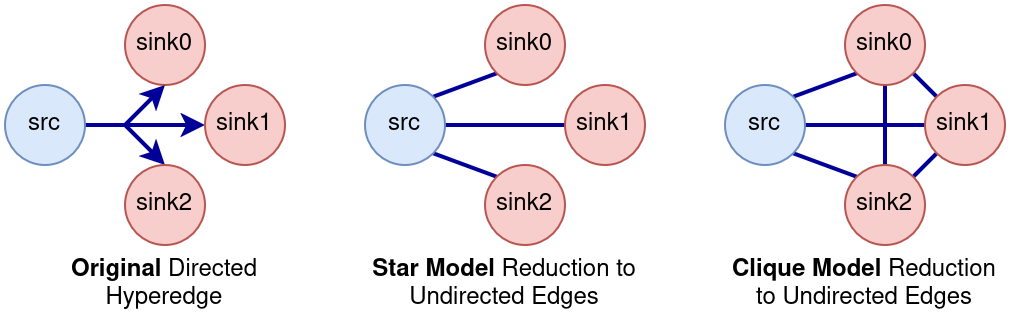
\includegraphics[width=\columnwidth]{figures/future_work/net_model.png}
    \captionof{figure}{Hyperedge reduction via Star and Clique net models.}
    \label{fig:net_model}
}
{
    \centering
    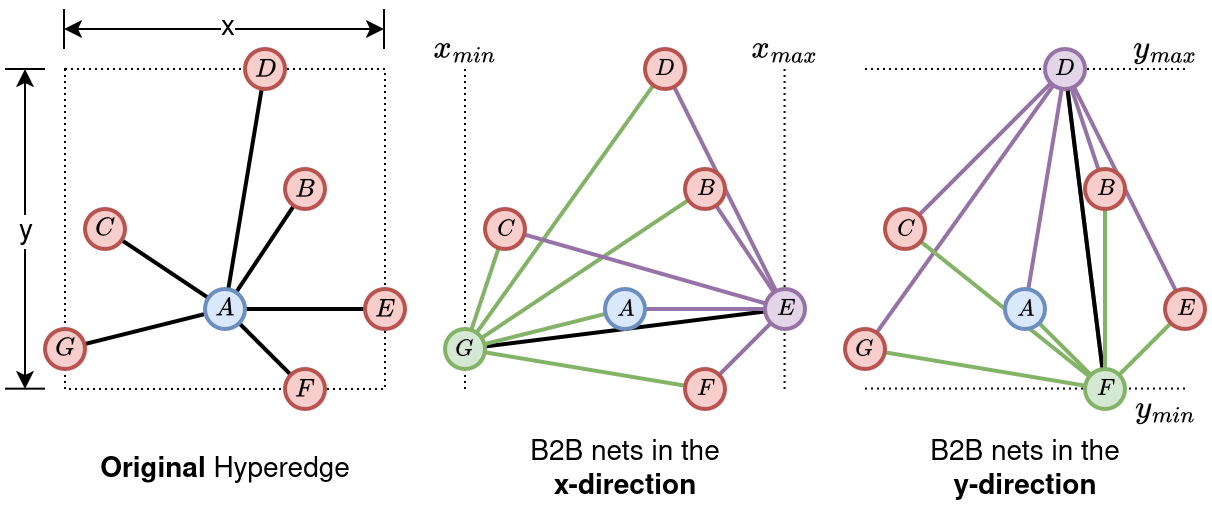
\includegraphics[width=\columnwidth]{figures/future_work/bound2bound.png}
    \captionof{figure}{Hyperedge reduction via Bound2Bound net model.}
    \label{fig:bound2bound}
}

After reduction comes global placement, where AP minimizes a wirelength objective, typically either a linear HPWL formulation \eqref{equ:Manhattan} or a quadratic approximation \eqref{equ:Euclidian}:


\begin{equation}
    \boldsymbol{\Phi} (\boldsymbol{x}, \boldsymbol{y}) = \sum_{i,j} w_{ij} \left( |x_i - x_j| + |y_i - y_j| \right)
    \label{equ:Manhattan}
\end{equation}

\begin{equation}
    \boldsymbol{\Phi} (\boldsymbol{x}, \boldsymbol{y}) = \sum_{i,j} w_{ij} \left[ (x_i - x_j)^2 + (y_i - y_j)^2 \right]
    \label{equ:Euclidian}
\end{equation}

with $i, j \in \{1, 2, ..., M\}$, where $M$ is the total number of modules in the design.
Module placements in the $x$ and $y$ directions are captured by the placement vectors \( \boldsymbol{x} = (x_1, x_2, ..., x_n) \) and \( \boldsymbol{y} = (y_1, y_2, ..., y_n) \), where $x_n$ and $y_n$ correspond to the coordinates of the $n$th module instance.
Edges connecting pins $i$ and $j$ have weights $w_{ij}$ and are assigned values depending on the selected net model and objective.

In both formulations, the objective function is separable with $x$ and $y$.
The squared objective is strongly convex and yields a unique minimizer while requiring a single linear solve per iteration. 
However, it tends to over-emphasize long wires relative to short ones and tends to worsen routing demand compared to linear metrics \cite{AP_2000}. 
The linear wirelength objective more closely reflects how HPWL is measured and better correlates with routability. 
However, it is non-differentiable, so analytical placers typically handle it by iterated quadratic approximations or by smooth regularizations that enable Newton-type solvers \cite{AP_2000}. 
For ease of implementation, it would be best to first implement the squared objective before exploring the linear objective.

We can use the FPGA placer HeAP (2012) \cite{AP_2012}, which uses the squared objective along with the B2B net model, as an instructive reference.
In HeAP, edges are weighted inversely with the distances between between pins and the number of pins on the original hyperedge from which the edge was produced.

\begin{equation}
    w_{ij} = \frac{2}{(p-1)\,|x_i - x_j|}.
    \label{equ:weight_linearized}
\end{equation}


The squared objective \ref{equ:Euclidian} can be recast into matrix-vector form.
In the x-direction this can be written as:
\begin{equation}
    \boldsymbol{\Phi} (\boldsymbol{x}) 
    = \tfrac{1}{2}\,\boldsymbol{x}^T \boldsymbol{Q}_x\,\boldsymbol{x} + \boldsymbol{c}_x^T \boldsymbol{x} + \text{const},
    \label{equ:quadratic}
\end{equation}

The connectivity matrix $\boldsymbol{Q_x}$ encodes 2-pin connections between movable instances while $\boldsymbol{c_x}$ encodes 2-pin connections between movable instances and fixed instances   
Movable instances are for example \texttt{SLICEL}s, DSP, and RAM, while fixed instances can be IO pads and clock buffers.
We distinguish fixed instances because their placement cannot be optimized and can be thought of as constraints encoded into the objective.
For a design with $M$ pins belonging to movable instances and $F$ pins belonging to fixed instances, $\boldsymbol{Q}_x \in {\mathbb{R}}^{M \times M}$ and $\boldsymbol{c}_x \in {\mathbb{R}}^F$.

Since the objective is strongly convex, we can solve for the global minimum cost by setting the partial derivatives to zero.

\begin{equation}
    \frac{\partial}{\partial x} \boldsymbol{\Phi} (\boldsymbol{x}) = 0 \Longleftrightarrow \boldsymbol{Q}_x \boldsymbol{x} = - \boldsymbol{c}_x
\end{equation}

Solving this linear system yields the optimal $x$ coordinate placements, and the same applies independently for $y$.
We can use any number of OTS solver frameworks for this step, potentially \texttt{cvxpy} in Python or a Java-native package like \texttt{EMJ}.
Note that this is only global placement, which is not legal and contains many constraint violations and placement overlaps.

Following global placement is detailed placement (legalization) which is where the real challenge begins.
Most placers have a custom method for doing so, tailored to specific optimizations or cost objectives.
We can continue using HeAP as a reference, which performs recursive partitioning to transform the solution provided by the solver into a legal overlap-free placement.
The discrete nature of the arrangement of \texttt{Site}s on the \texttt{device} and all of the other hardware constraints will make implementation very difficult.
Just like in our SA placer, the most challenging parts to implement were the prepacker and packer where we deal with placement constraints, not the placer itself.

% The first step of legalization is to identify areas or \texttt{Site}s on the \texttt{device} that are overutilized.
% If we take the global placement containing the ($x$, $y$) coordinates of all instances, overlay it onto the grid of resources of the \texttt{device}, and snap each instance to the closest legal \texttt{Site}, any \texttt{Site} occupied by more than one instance can be considered overutilized.
% Overutilized \texttt{Site}s that are adjacent to one another are repeatedly clustered together until all clusters are bordered on all sides by non-overutilized \texttt{Site}s, giving us so-called "overutilized areas".
% Next, each area is expanded in both $x$ and $y$ dimensions until it is large enough to accomodate all instances within.
% 
% In the second step, we generate two cuts: source cut and a target cut.
% The source cut pertains to the instances being placed and the target cut pertains to the area of \texttt{Site}s into which the instances are placed.
% This is a similar to our SA placer when making random moves and swaps, where we have an original "home" \texttt{Site} and a proposed "away" \texttt{Site} that we accept or reject based on cost and temperature, except now we are dealing with clusters of \texttt{Site}s which are non-uniform in shape.
% The source cut splits the instances into two partitions, while the target cut splits the area into two sub-areas, into which the instances in each partition are spread.
% The target cut is a horizontal $x$ or vertical $y$ cut of the area such that all blocks in each partition fit in their respective sub-areas.
% 
% Next, the instances in sub-areas are spread to distribute them evenly.
% The discrete nature of FPGA \texttt{Site} locations will make this process difficult.







% We know the squared objective function \ref{equ:Euclidian} to be strongly convex and quadratic, so it would be beneficial to be able to re-express it in matrix-vector form to easily access gradient and Hessian information about the system and to make it compatible with OTS solvers.
% With some algebraic manipulation, we can cast sum of squares formulation (\ref{equ:Euclidian}) into quadratic matrix form.
% Take the original objective in the x-direction:
% 
% \begin{equation}
%     {\boldsymbol{\Phi}}_x (\boldsymbol{x}) = \sum_{i, j} w_{ij} \left( x_i - x_j \right)^2
%     \label{equ:sq_obj_x}
% \end{equation}
% 
% Expanding the summation:
% 
% \begin{equation}
%     {\boldsymbol{\Phi}}_x (\boldsymbol{x}) = \sum_{i, j} w_{ij} x_i^2 + \sum_{i, j} w_{ij} x_j^2 - 2 \sum_{i, j} w_{ij} x_i x_j
%     \label{equ:w_expand}
% \end{equation}
% 
% A net connecting node $i$ with $j$ is the same as connecting node $j$ with $i$, so $w_{ij} = w_{ji}$.
% This means the weight matrix $W$ with elements $w_{ij}$ is symmetric.
% Using this symmetry, we can group the first two terms in \ref{equ:w_expand}:
% \begin{equation}
%     {\boldsymbol{\Phi}}_x (\boldsymbol{x}) = 2 \sum_{i, j} w_{ij} x_i^2  - 2 \sum_{i, j} w_{ij} x_i x_j
%     \label{equ:w_grouped} 
% \end{equation}



% by constructing the \emph{graph Laplacian matrix} out of the undirected weighted graph $G = (V, E)$ after hypergraph reduction. 
% 
% The Laplacian matrix \(L\) can be constructed with:
% 
% \begin{equation}
%     L = BWB^T
% \end{equation}
% 
% where $B$ is the \emph{incidence matrix} and $W$ is the diagonal \emph{weight matrix}.
% The $|v| \times |e|$ incidence matrix $B$ of graph $G$ has elements $b_{ve}$, where $v$ denotes the vertex index and $e$ denotes the edge index.
% Each edge $e$ connects a head vertex and a tail vertex, denoted as $e = (v_{head}, v_{tail})$.
% 
% \begin{equation}
%     b_{ve} = 
%     \begin{cases}
%         +1, & \text{if } v \text{ is the head (source) of edge e} \\
%         -1, & \text{if } v \text{ is the tail (sink) of edge e} \\ 
%         0, & \text{otherwise}.
%     \end{cases}
% \end{equation}
% 
% The assignment of which vertex is the head and which is the tail is arbitrary and does not correlate with any directionality of the edges.
% But for consistent bookkeeping purposes, we can assign the lower-indexed vertex as the head and the higher-indexed vertex as the tail like so: 
% 
% \begin{equation}
%     b_{ve} = 
%     \begin{cases}
%         +1, & \text{if } v = v_i, \\
%         -1, & \text{if } v = v_j, \\ 
%         0, & \text{otherwise}.
%     \end{cases}
% \end{equation}



\subsection{Variations on Packing}
Our current placer follows a \textbf{Site-centric} approach that resembles that of the old Xilinx ISE - the predecessor to Vivado used in the 2000s.
These days, Vivado performs \textbf{BEL-centric} placement without necessarily locking \texttt{Cell}s into \texttt{Site}s, allowing for a higher granularity of movement of \texttt{Cell}s. 
Enabling BEL-centric moveme
nt as opposed to Site-centric movement can improve HPWL minimization, but will add much more complexity to the packing and placement process to ensure robustness with respect to hardware constraints, particularly with intra-\texttt{Site} routing.

There is no constraint that forces us to pack \texttt{Cells} into \texttt{SiteInst}s before placement or to follow a strict prepacking-packing-placement flow. 
After implementing a force-directed or analytical placer, we can begin to explore different packing and placement ordering like those studied in Wuxi et al. (2019) \cite{ExplicitPacking}.

{
    \centering
    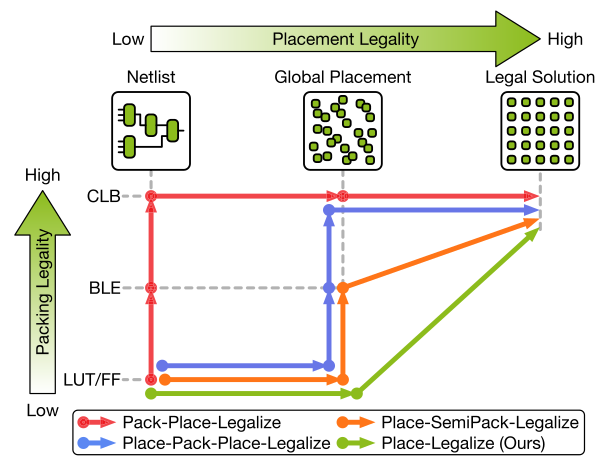
\includegraphics[width=\columnwidth]{figures/future_work/legalization.png}
    \captionof{figure}{Representative FPGA placement and packing flows. Figure taken from Wuxi et al. (2019), page 1 \cite{ExplicitPacking}}
}
\vspace{0.25cm}

\subsection{Add Hard Macro Support}
As mentioned before, our SA placer is Site-centric.
An interesting direction of study would be to expand our placer to support Module-Site-centric mixed placement, where Modules are hard macros comprising multiple Sites.
This of course would also add complexity to the prepacker and packer, as now we are dealing with non-uniform mixed-size placement objects.
The RapidWright repository has two implementations of purely Module-centric placers, called \texttt{BlockPlacer} and \texttt{BlockPlacer2}, though it currently lacks a purely Site-centric placer or a mixed Module-Site-centric placer.
The corresponding paper by Lavin et. al. (2010) \cite{HardBlock} can serve as a useful reference for this direction.



